
\section{Introduction}

This appendix provides a few foundational mathematical concepts in a very brief and focused way for review. The following sections will introduce vector and matrix algebra, basic concepts of probability and random variables, and finally core concepts of differential calculus. These concepts are usually taught in introductory courses and are provided here in very concise form as a review.

\begin{resourcebox}
A deeper treatment of the material in this appendix is available in many introductory textbooks, for example in this one:\\


Kevin P. Murphy: \emph{Probabilistic Machine Learning -- An Introduction}. The MIT Press, Camridge, MA, 2022.

\small\url{https://probml.github.io/pml-book/book1.html}\normalsize \\

Chapters 1, 2, and 7
\end{resourcebox}

\section{Vectors}

A \index{Vector}\emph{vector} is a list of numbers. Vectors are useful to express the same calculation involving multiple numbers. For example, data that consists of 1000 measurements of people's height can be expressed as a $1000 \times 1$ vector. Then, doing arithmetic with these numbers is much easier to write than writing out the same equation 1000 times. 

For example, the vector

\begin{align*}
\mathbf{A} = \begin{pmatrix}3 \\ 1 \\ 4 \\ -1\end{pmatrix}
\end{align*}

is a \emph{column vector} (or vertical vector) of four integer numbers. It has \index{Dimensionality (of a vector)}\emph{dimensionality} of $4 \times 1$, that is, it has 4 rows and 1 column. Usually, vectors are written with round brackets as done here, but some authors use square bracket notation. 

There are different conventions to indicate that a variable is a vector; the above example has written the vector in bold font and capitalized as $\mathbf{A}$, sometimes it is written with a superscript arrow like $\overrightarrow{A}$ or $\overrightarrow{a}$ and some authors reserve capital letters for matrices (see below), using lower-case letters for vectors. Sometimes it is useful to indicate the dimensionality of a vector, typically written in subscript form like $\mathbf{_4 A _1}$ or $\mathbf{A_{4 \times 1}}$. 

The elements of a vector are identified by their position as subscript, and are sometimes written as lower-case variables or as non-bold variables, for example: $A_1 = 3$ or $a_1 = 3$.

We define another vector like this:
\begin{align*}
\mathbf{B} = \begin{pmatrix}2 & -2 & 1 & 3\end{pmatrix}
\end{align*}

The vector $\mathbf{B}$ is a \emph{row vector} (or horizontal vector) with dimensionality $1 \times 4$, that is, it has 1 row and 4 columns.

To transform a horizontal vector into a vertical one, or vice versa, one uses the \index{Transpose}\emph{transpose} operation, typically indicated by a superscript $T$ like $\mathbf{A}^T$ or a ''prime'' symbol, like $\mathbf{A}'$. The transpose ''flips'' the rows and columns:

\begin{align*}
\mathbf{A}^T = \begin{pmatrix}3 & 1 & 4 & -1\end{pmatrix} \qquad
\mathbf{B}^T = \begin{pmatrix}2 \\ -2 \\ 1 \\ 3 \end{pmatrix}
\end{align*}

Basic arithmetic of vectors and scalars (that is, vectors of dimension $1 \times 1$, that is, simple numbers) is done element-wise. For example:

\begin{align*}
\mathbf{A} + 2 = \begin{pmatrix}5 \\ 3 \\ 6 \\ 1 \end{pmatrix} \qquad
\mathbf{A} \cdot 5 = \begin{pmatrix}15 \\ 5 \\ 20 \\ -5\end{pmatrix}
\end{align*}

Vector addition is also done element-wise if the dimensions of the two vectors are the same. For example,
\begin{align*}
\mathbf{A} + \mathbf{B}^T = \begin{pmatrix}3 &+& 2 \\
1 &+& -2 \\
4 &+& 1 \\
-1 &+& 3 \end{pmatrix} = \begin{pmatrix}5 \\ -1 \\ 5 \\ 2 \end{pmatrix}
\end{align*}

The \index{Dot product}\emph{dot product} or \emph{inner product} of two vectors is defined between a row vector and a column vector of equal length. The resulting vector will be a scalar (that is, a simple number) defined as the sum of the products of the corresponding elements of the two vectors. That is, multiply the first element of the row vector with the first element of the column vector, then the second elements, and so on. Then, sum all the products. For example:

\begin{align*}
\mathbf{B} \cdot \mathbf{A} &= \begin{pmatrix}2 & -2 & 1 & 3\end{pmatrix} \cdot \begin{pmatrix}3 \\ 1 \\ 4 \\ -1\end{pmatrix} \\
&= 2 \times 3 + (-2) \times 1 + 1 \times 4 + 3 \times (-1) = 5
\end{align*}

With this, the square of a vector can be defined as
\begin{align*}
\mathbf{A}^2 = \mathbf{A}^T \cdot \mathbf{A} = 9 + 1 + 16 + 1 = 27
\end{align*}

The \emph{outer product} of two vectors $\mathbf{A} \otimes \mathbf{B}$ is computed by multiplying the first vector by each element of the second vector to yield multiple column vectors. This result is called a \emph{matrix}, discussed below:

\begin{align}
\mathbf{A} \otimes \mathbf{B} &= \begin{pmatrix}3 \\ 1 \\ 4 \\ -1\end{pmatrix} \otimes \begin{pmatrix}2 & -2 & 1 & 3\end{pmatrix}\nonumber \\
&= \begin{pmatrix}3 \times  2 & 3 \times -2 & 3 \times 1 & 3 \times 3 \\
1 \times  2 & 1 \times -2 & 1 \times 1 & 1 \times 3 \\
4 \times  2 & 4 \times -2 & 4 \times 1 & 4 \times 3 \\
-1 \times  2 & -1 \times -2 & -1 \times 1 & -1 \times 3 \end{pmatrix} \nonumber \\
&= \begin{pmatrix}6 & -6 & 3 & 9 \\
2 & -2 & 1 & 3 \\
8 & -8 & 4 & 12 \\
-2 & 2 & -1 & -3 \end{pmatrix} \label{eq:matrix1}
\end{align}

In the above example, the outer product $\mathbf{A} \otimes \mathbf{B}$ results in a matrix of dimensionality $4 \times 4$, that is, it has 4 rows and 4 columns. More on matrices below.

The \emph{norm}\index{Norm (of a vector)} of a vector is a measure of its ''length''. In general, the \emph{p-norm} of a vector is defined as follows (the notation $|x|$ means the absolute value of $x$):

\begin{align*}
||\mathbf{A}||_p = \left( \sum_{i=1}^n |a_i|^p \right) ^{1/p}
\end{align*}

Typical norms are the \emph{absolute norm} or 1-norm where $p=1$:

\begin{align*}
||\mathbf{A}||_1 = \left( \sum_{i=1}^n |a_i| \right)
\end{align*}

\noindent or the \emph{Euclidean norm} or 2-norm where $p=2$:

\begin{align*}
||\mathbf{A}||_2 &= \left( \sum_{i=1}^n a_i^2 \right) ^{1/2} \\
&= \sqrt{ \sum_{i=1}^n a_i^2 } \\ 
&= \sqrt{ \mathbf{A}^T \cdot \mathbf{A}}
\intertext{such that}
||\mathbf{A}||_2^2 &= \mathbf{A}^T \cdot \mathbf{A}
\end{align*}

Do not confuse the superscripts and subscripts on $||\mathbf{A}||^2_2$ and do not confuse the norm $||.||$ with the absolute value $|.|$ notation. 

\section{Matrices}

A \emph{matrix}\index{Matrix} $\mathbf{C}$ with $m$ rows and $n$ columns, that is, of dimensionality $m \times n$, is a two-dimensional array of numbers. The first index counts the rows, the second index the columns. For example:

\begin{align*}
\mathbf{C} = \begin{pmatrix}c_{11} & c_{12} & \cdots & c_{1n} \\
c_{21} & c_{22} & \cdots & c{2n} \\
\vdots & \vdots & \ddots & \vdots \\
c_{m1} & c_{m2} & \cdots & c_{mn} \end{pmatrix}
\end{align*}

An example $4 \times 4$ matrix is that in Equation~\ref{eq:matrix1} above, repeated here:

\begin{align*}
\mathbf{C} = \begin{pmatrix}6 & -6 & 3 & 9 \\
2 & -2 & 1 & 3 \\
8 & -8 & 4 & 12 \\
-2 & 2 & -1 & -3 \end{pmatrix}
\end{align*}

As for vectors above, the \emph{transpose} operation again ''flips'' the rows and columns, such that:

\begin{align*}
\mathbf{C}^T = \begin{pmatrix}
6 & 2 & 8 & -2 \\
-6 & -2 & -8 & 2 \\
3 & 1 & 4 & -1 \\
9 & 3 & 12 & -3 \end{pmatrix}
\end{align*}

Operations between matrices and scalars are defined element-wise, the same as they are for operations between vectors and scalars. For example:

\begin{align*}
\mathbf{C} + 2 &= \begin{pmatrix}8 & -4 & 5 & 11 \\
4 & 0 & 3 & 5 \\
10 & -6 & 6 & 14 \\
0 & 4 & 1 & -1 \end{pmatrix} \\ 
\mathbf{C} \cdot 5 &= \begin{pmatrix}30 & -30 & 15 & 45 \\
10 & -10 & 5 & 15 \\
60 & -40 & 20 & 60 \\
-10 & 10 & -5 & -15 \end{pmatrix}
\end{align*}

Matrix addition is defined element-wise only if the dimensions of the two matrices are identical. For example:

\begin{align*}
\begin{pmatrix}1 & 2 \\ 3 & 4\end{pmatrix} + \begin{pmatrix}5 & 6 \\ 7 & 8\end{pmatrix} = \begin{pmatrix}6 & 8 \\ 10 & 14\end{pmatrix}
\end{align*}

Multiplication of two matrices is defined if the left matrix has as many columns as the right matrix has rows. The product of two matrices $\mathbf{A}_{m \times n}$ and $\mathbf{B}_{n \times p}$ is a matrix $\mathbf{C}_{m \times p}$ where each element of $\mathbf{C}$ is defined as:

\begin{align*}
C_{ij} = \sum_{k=1}^n A_{ik} B_{kj}
\end{align*}

For example, let 
\begin{align*}
\mathbf{A}_{3\times 2} &= \begin{pmatrix}1 & 2 \\
3 & 4 \\
5 & 6 \end{pmatrix} 
\intertext{and}
\mathbf{B}_{2 \times 4} &= \begin{pmatrix}-2 & 0 & 2 & 4 \\
-1 & 3 & 7 & 11 \end{pmatrix}
\intertext{then}
\mathbf{C}_{3 \times 4} &= \mathbf{A}_{3\times 2} \otimes \mathbf{B}_{2\times 4} \\
&= \begin{pmatrix}
1\cdot -2+2\cdot -1 & 1\cdot 0 + 2 \cdot 3 & 1 \cdot 2 + 2 \cdot 7 & 1 \cdot 4 + 2 \cdot 11 \\
3 \cdot -2 + 4 \cdot -1 & 3 \cdot 0 + 4 \cdot 3 & 3 \cdot 2 + 4 \cdot 7 & 3 \cdot 4 + 4 \cdot 11 \\
5 \cdot -2 + 6 \cdot -1 & 5 \cdot 0 + 6 \cdot 3 & 5 \cdot 2 + 6 \cdot 7 & 5 \cdot 4 + 6 \cdot 11 \end{pmatrix} \\
&= \begin{pmatrix}
-4 & 6 & 16 & 26 \\
-10 & 12 & 34 & 56 \\
-16 & 18 & 52 & 86 \end{pmatrix}
\end{align*}


\begin{infobox}
The matrix product is defined only if the dimensionalities of the two matrices match. Understanding how the dimensions of the resulting matrix is a function of the dimensions of the left and right factor of the matrix multiplication is useful to verify the correctness of matrix operations.

\vspace{.5\baselineskip}

For example, if you know the result should be a scalar, that is, a $1 \times 1$ matrix, you can use the dimensionalities of the two factors to verify this. Similarly, if you know the result should be a column vector, that is, a $m \times 1$ matrix, you can make sure the dimensionalities of the factors of a matrix multiplication are correct to give this result.
\end{infobox}

There are three useful properties of matrix multiplication:

\begin{enumerate}
\item Matrix multiplication is \emph{associative}: $\mathbf{(AB)C = A(BC)}$. In other words, it does not matter where you begin to multiply.
\item Matrix multiplication is \emph{distributive}: $\mathbf{A(B + C) = AB + AC}$. In other words, it does not matter whether you add first, and then multiply, or whether you multiply first, and then add.
\item Matrix multiplication is usually \emph{not commutative}: $\mathbf{AB \neq BA}$. In other words, it does matter which way around you multiply the matrices.
\end{enumerate}

Even though this chapter introduces vectors before matrices, vectors can best be thought of as special types of matrices, with either a single column (column vector) or a single row (row vector). As such, the associative and distributive properties also hold for vectors. 

\section{Probability}

Let $E$ be some event, then $\operatorname*{Pr}(E)$, also sometimes written simply as $p(E)$, is the probability that event $E$ occurs. By definition:

\begin{align*}
0 \leq \operatorname*{Pr}(E) \leq 1
\end{align*}

For the complementary event $\neg E$ (''not E''), the probability of occurrence then is:

\begin{align*}
\operatorname*{Pr}(\neg E) = 1 - \operatorname*{Pr}(E)
\end{align*}

The \emph{joint probability} of two events $E$ and $F$ occurring together, that is, the probability of the intersection of two events, is defined as follows:

\begin{align}
\operatorname*{Pr}(E \wedge F) &= \operatorname*{Pr}(E, F) \nonumber
\intertext{and for the special case of \emph{independent events} $E$ and $F$:}
\operatorname*{Pr}(E \wedge F) &= \operatorname*{Pr}(E) \cdot \operatorname*{Pr}(F) \label{eq:prob1}
\end{align}

For example, when rolling two dice, with $E$ denoting the event that the first dice turns up 5 and $F$ denoting the event that the second dice turns up 2, the two events $E$ and $F$ are independent, each occurring with probability $1/6$. The joint probability of both $E$ and $F$ occurring is then $1/6 \cdot 1/6 = 1/36$. In fact, Equation~\ref{eq:prob1} is how the independence of events is \emph{defined}.

The probability of events $E$ or $F$ occurring, that is, the probability of the union of two events, is given by

\begin{align*}
\operatorname*{Pr}(E \vee F) &= \operatorname*{Pr}(E) + \operatorname*{Pr}(F) - \operatorname*{Pr}(E \wedge F)
\intertext{and for the special case of \emph{mutually exclusive events} for which $\operatorname*{Pr}(E \wedge F)=0$:}
\operatorname*{Pr}(E \vee F) &= \operatorname*{Pr}(E) + \operatorname*{Pr}(F)
\end{align*}

For example, the probability of a dice showing the number 1 or the number 3 is $1/6 + 1/6 = 1/3$ because the two events are mutually exclusive, that is, the dice cannot show both numbers.

The \emph{conditional probability} of event $E$ occurring, given that event $F$ has occurred, that is, under the condition that $F$ has occurred, is defined as:

\begin{align}
\operatorname*{Pr}(E | F) = \frac{\operatorname*{Pr}(E, F)}{\operatorname*{Pr}(F)} \nonumber
\intertext{or, rearranged}
\operatorname*{Pr}(E, F) = \operatorname*{Pr}(E | F) \operatorname*{Pr}(F) \label{eq:prob2}
\end{align}

Equation~\ref{eq:prob2} is called the \emph{product rule of probability} and is useful in the following application. First, note that
\begin{align}
\operatorname*{Pr}(E, F) &= \operatorname*{Pr}(F, E) \nonumber
\intertext{then, by applying Equation~\ref{eq:prob2} on both sides:}
\operatorname*{Pr}(E | F) \operatorname*{Pr}(F)  &= \operatorname*{Pr}(F | E) \operatorname*{Pr}(E) \nonumber
\intertext{rearranging:}
\operatorname*{Pr}(E | F) &= \frac{\operatorname*{Pr}(F | E) \operatorname*{Pr}(E)}{\operatorname*{Pr}(F)} \label{eq:prob3}
\end{align}

\begin{infobox}
Equation~\ref{eq:prob3} is known as \emph{Bayes' theorem}\index{Bayes' theorem} after the Reverend Thomas Bayes (1702--1761), an English mathematician and minister. 

\vspace{.5\baselineskip}
Bayes' theorem is most often used to describe updating of probabilities or ''beliefs'' after observing some evidence. In this context, $\operatorname*{Pr}(E)$ is called the \emph{prior probability} or just the \emph{prior} of observing event $E$, while $\operatorname*{Pr}(F | E)$ is the \emph{likelihood} of observing event $F$ (the ''evidence'') just in case that condition $E$ holds. The resulting $\operatorname*{Pr}(E | F)$ is the \emph{posterior probability} of observing event $E$ after observing the evidence $F$. 
\end{infobox}

For example, let $F$ be the event ''smoke'' and $E$ be the event ''fire''. Then, in any given situation $\operatorname*{Pr}(E)$ is quite small, for example, $0.05$; one does not normally expect to see fire. However, one can intuit that $\operatorname*{Pr}(F | E)$ is quite high as most fires produce smoke, for example, $0.95$. To calculate $\operatorname*{Pr}(E | F)$, the probability of ''fire'' conditional on having observed ''smoke'', one needs $\operatorname*{Pr}(F)$, which can be computed as follows:

\begin{align*}
\operatorname*{Pr}(F) = \operatorname*{Pr}(F | E) \operatorname*{Pr}(E) + \operatorname*{Pr}(F | \neg E)\operatorname*{Pr}(\neg E)
\end{align*}

For example, with $\operatorname*{Pr}(F | \neg E) = 0.01$ (the probability of observing smoke without fire is quite small) and $\operatorname*{Pr}(\neg E) = 1 - \operatorname*{Pr}(E)$:

\begin{align*}
\operatorname*{Pr}(F) = 0.95 \cdot 0.05 + 0.01 \cdot 0.95 = 0.95 \cdot 0.06 = 0.057
\end{align*}

Then the probability of ''fire'' (E) having observed ''smoke'' (F) is:

\begin{align*}
\operatorname*{Pr}(E | F) &= \frac{\operatorname*{Pr}(F | E) \operatorname*{Pr}(E)}{\operatorname*{Pr}(F)} \\
&= \frac{0.95 \cdot 0.05}{0.057} = 0.833
\end{align*}

\section{Random Variables}

A \emph{random variable}\index{Random variable} $X$ is a variable that takes on values $x_i$ of its domain with some probability $\operatorname*{Pr}(X=x_i)$. Random variables may be discrete, that is, they can take on only certain values, or they may be continuous, that is, they may take on any real value. 

The \emph{expected value}\index{Expected value} of a random variable, written as $\mathbb{E}(X)$, as $\operatorname*{Exp}(X)$, or sometimes as $\mu$ (but not to be confused with the mean, also sometimes denoted as $\mu$), is defined as follows, where $i$ indexes the entire domain of $X$, that is, the following sum or integral is over all possible values of $X$ (in the following, we write the probability as $p(\cdot)$, rather than $\operatorname*{Pr}(\cdot)$).

\begin{align*}
\mathbb{E}(X) &= \sum_i x_i \cdot p(X=x_i) \qquad \text{(for discrete variables)}
\intertext{or}
\mathbb{E}(X) &= \int_i x_i \cdot p(X=x_i) dx \qquad \text{(for continuous variables)}
\end{align*}

In other words, the expected value or ''expectation'' is the sum of the possible values, weighted by their probability. For example, the expected value of a discrete random variable $R$ representing the roll of a dice can be shown as:
\begin{align*}
\mathbb{E}(R) = 1/6 \cdot 1 + 1/6 \cdot 2 + 1/6 \cdot 3 + 1/6 \cdot 4 + 1/6 \cdot 5 + 1/6 \cdot 6 = 3.5
\end{align*}

The expectation is a linear operator, that is

\begin{align*}
\mathbb{E}(aX + b) = a \mathbb{E}(X) + b
\end{align*}

\noindent where $a$ and $b$ are scalars and $X$ is a random variable.

Linearity also extends to the sum of $n$ random variables, such that the expectation of the sum is the sum of the expectations:

\begin{align*}
\mathbb{E} \left( \sum_{i=1}^n X_i \right) = \sum_{i=1}^n \mathbb{E}(X_i)
\end{align*}

For example, the expectation of the sum of two random variables $R_1$ and $R_2$ representing the rolls of two independent dice is:

\begin{align*}
\mathbb{E}(R_1 + R_2) = \mathbb{E}(R_1) + \mathbb{E}(R_2) = 3.5 + 3.5 = 7
\end{align*}

This result can be verified using the probability for joint events above and enumerating all possible combinations of two dice rolls.

For $n$ independent random variables, the expectation of their product is the product of their expectations:

\begin{align*}
\mathbb{E} \left( \prod_{i=1}^n X_i \right) = \prod_{i=1}^n \mathbb{E}(X_i)
\end{align*}

The \emph{variance}\index{Variance} of a random variable measures how far the values of a variable are ''spread out'' around the expectation. It is often denoted by the symbol $\sigma^2$, or written as $\mathbb{V}(X)$ or $\operatorname*{Var}(X)$ and defined as follows:

\begin{align*}
\mathbb{V}(X) = \operatorname*{Var}(X) = \sigma^2(X) &= \mathbb{E}\left[ (X - \mathbb{E}(X))^2 \right]
\intertext{With a little algebra, for the discrete case:}
&= \sum_i (x_i - \mathbb{E}(X))^2 p(x_i) \\ 
&= \sum_i (x_i^2 + \mathbb{E}(X)^2 - 2 \mathbb{E}(X) x_i) p(x_i) \\
&= \sum_i x_i^2 p(x_i) + \mathbb{E}(X)^2 \sum_i p(x_i) - 2 \mathbb{E}(X) \sum_i x_i p(x_i) \\
\intertext{since $\sum_i p(x_i) = 1$ in the second term (probabilities sum to 1) and $\sum_i x_i p(x_i) = \mathbb{E}(X)$ in the third term:} 
&= \mathbb{E}(X^2) + \mathbb{E}(X)^2 - 2 \mathbb{E}(X) \mathbb{E}(X)  \\
&= \mathbb{E}(X^2) + \mathbb{E}(X)^2 - 2 \mathbb{E}(X)^2 \\
&= \mathbb{E}(X^2) - \mathbb{E}(X)^2
\end{align*}

The case for continuous variables can be shown in the same way, using integrals instead of sums.

For example, the variance of a random variable $R$ representing the roll of a dice is:

\begin{align*}
\mathbb{V}(R) &= \frac{1}{6} (1-3.5)^2 + \frac{1}{6} (2-3.5)^2 + \frac{1}{6} (3-3.5)^2 \\
& \qquad + \frac{1}{6} (4-3.5)^2 + \frac{1}{6} (5 - 3.5)^2 + \frac{1}{6} (6 - 3.5^2) \\
&= \frac{1}{6} \left[ (-5/2)^2 + (-3/2)^2 + (-1/2)^2 + (1/2)^2 + (3/2)^2 + (5/2)^2 \right] \\
&= \frac{1}{6} \left[ 25/4 + 9/4 + 1/4 + 1/4 + 9/4 + 25/4 \right] = 1/6 \cdot 70/4 = 70/24 \\
&= 35/12 
\end{align*}

The \emph{standard deviation}\index{Standard deviation} of a random variable is defined as the square root of the variance:

\begin{align*}
\operatorname*{std}(X) = \sigma(X) = \sqrt{\mathbb{V}(X)}
\end{align*}

The variance of a random variable $X$ multiplied by a scaling factor $a$ and shifted by an amount $b$ is:

\begin{align*}
\mathbb{V}(aX + b) = a^2 \mathbb{V}
\end{align*}

The variance of the sum of $n$ \emph{independent} random variables is the sum of their variances, that is:

\begin{align*}
\mathbb{V} \left[ \sum_{i=1}^n X_i \right] = \sum_{i=1}^n \mathbb{V}(X_i)
\end{align*}

For two random variables, one can define the \emph{covariance}\index{Covariance} as a generalization of the variance for a single variable. As the name implies, the covariance expresses the extent to which the two variables vary together, that is, how much does the other variable change when one variable changes. 

\begin{align*}
\operatorname*{Cov}(X, Y) &= \mathbb{E} \left[ (X - \mathbb{E}(X)) (Y - \mathbb{E}(Y) \right] \\
&= \mathbb{E}(XY) - \mathbb{E}(X)\mathbb{E}(Y)
\end{align*}

The covariance ranges between negative and positive infinity. Often, it is useful to have a measure with a lower and upper bound. For this, one divides the covariance by the square root of the product of the two variances. This quantity is called the \emph{correlation}\index{Correlation}, sometimes denoted as $\rho$ and ranges between $-1$ and $1$:

\begin{align*}
\rho = \operatorname*{Corr}(X, Y) = \frac{\operatorname*{Cov}(X, Y)}{\sqrt{\mathbb{V}(X) \mathbb{V}(Y)}}
\end{align*}


\begin{infobox}
There is often some confusion about what the covariance and correlation indicate. Note the following important points:

\begin{itemize}
\item Independent variables have zero covariance, but zero covariance does not imply that the variables are independent.
\item The correlation indicates the ''noiseness'' of the relation between two variables.
\item The correlation does not reflect the slope of the relationship between the two variables.
\item The correlation or covariance do not take into account non-linear relationships. 
\item Correlation does imply causation, but causation does imply correlation. 
\end{itemize}

\end{infobox}

Some of these points are illustrated in Figure~\ref{fig:math2}, showing different data sets of two variables and their correlation. The top row shows that the correlation indicates how ''noisy'' the relationship is; the slope of the relationship is the same for the data sets in the top row but the ''noisness'' changes with the the value of the correlation. The middle row shows that correlation does not indicate the slope of the relationship between the variables, as all data sets have the same correlation but clearly different slope of the relationship. The final row indicates different non-linear relationships that all have zero correlation. 

\begin{figure}
\centering

\includegraphics[width=.9\textwidth]{screen2.png} \\

\scriptsize Source: Murphy Figure 3.1 \\ \vspace{3mm}
\normalsize
\caption[Correlation and regression slopes]{Datasets and their correlations}
\label{fig:math2}
\end{figure}


\FloatBarrier


\section{Differential Calculus}

In differential calculus, the \emph{derivative} $f'$ of a function $f$ of some variable $x$ represents the slope of the tangent to the curve of the function $f$ at a particular position $x=x_0$, as shown in Figure~\ref{fig:math1}.

\begin{figure}
\centering
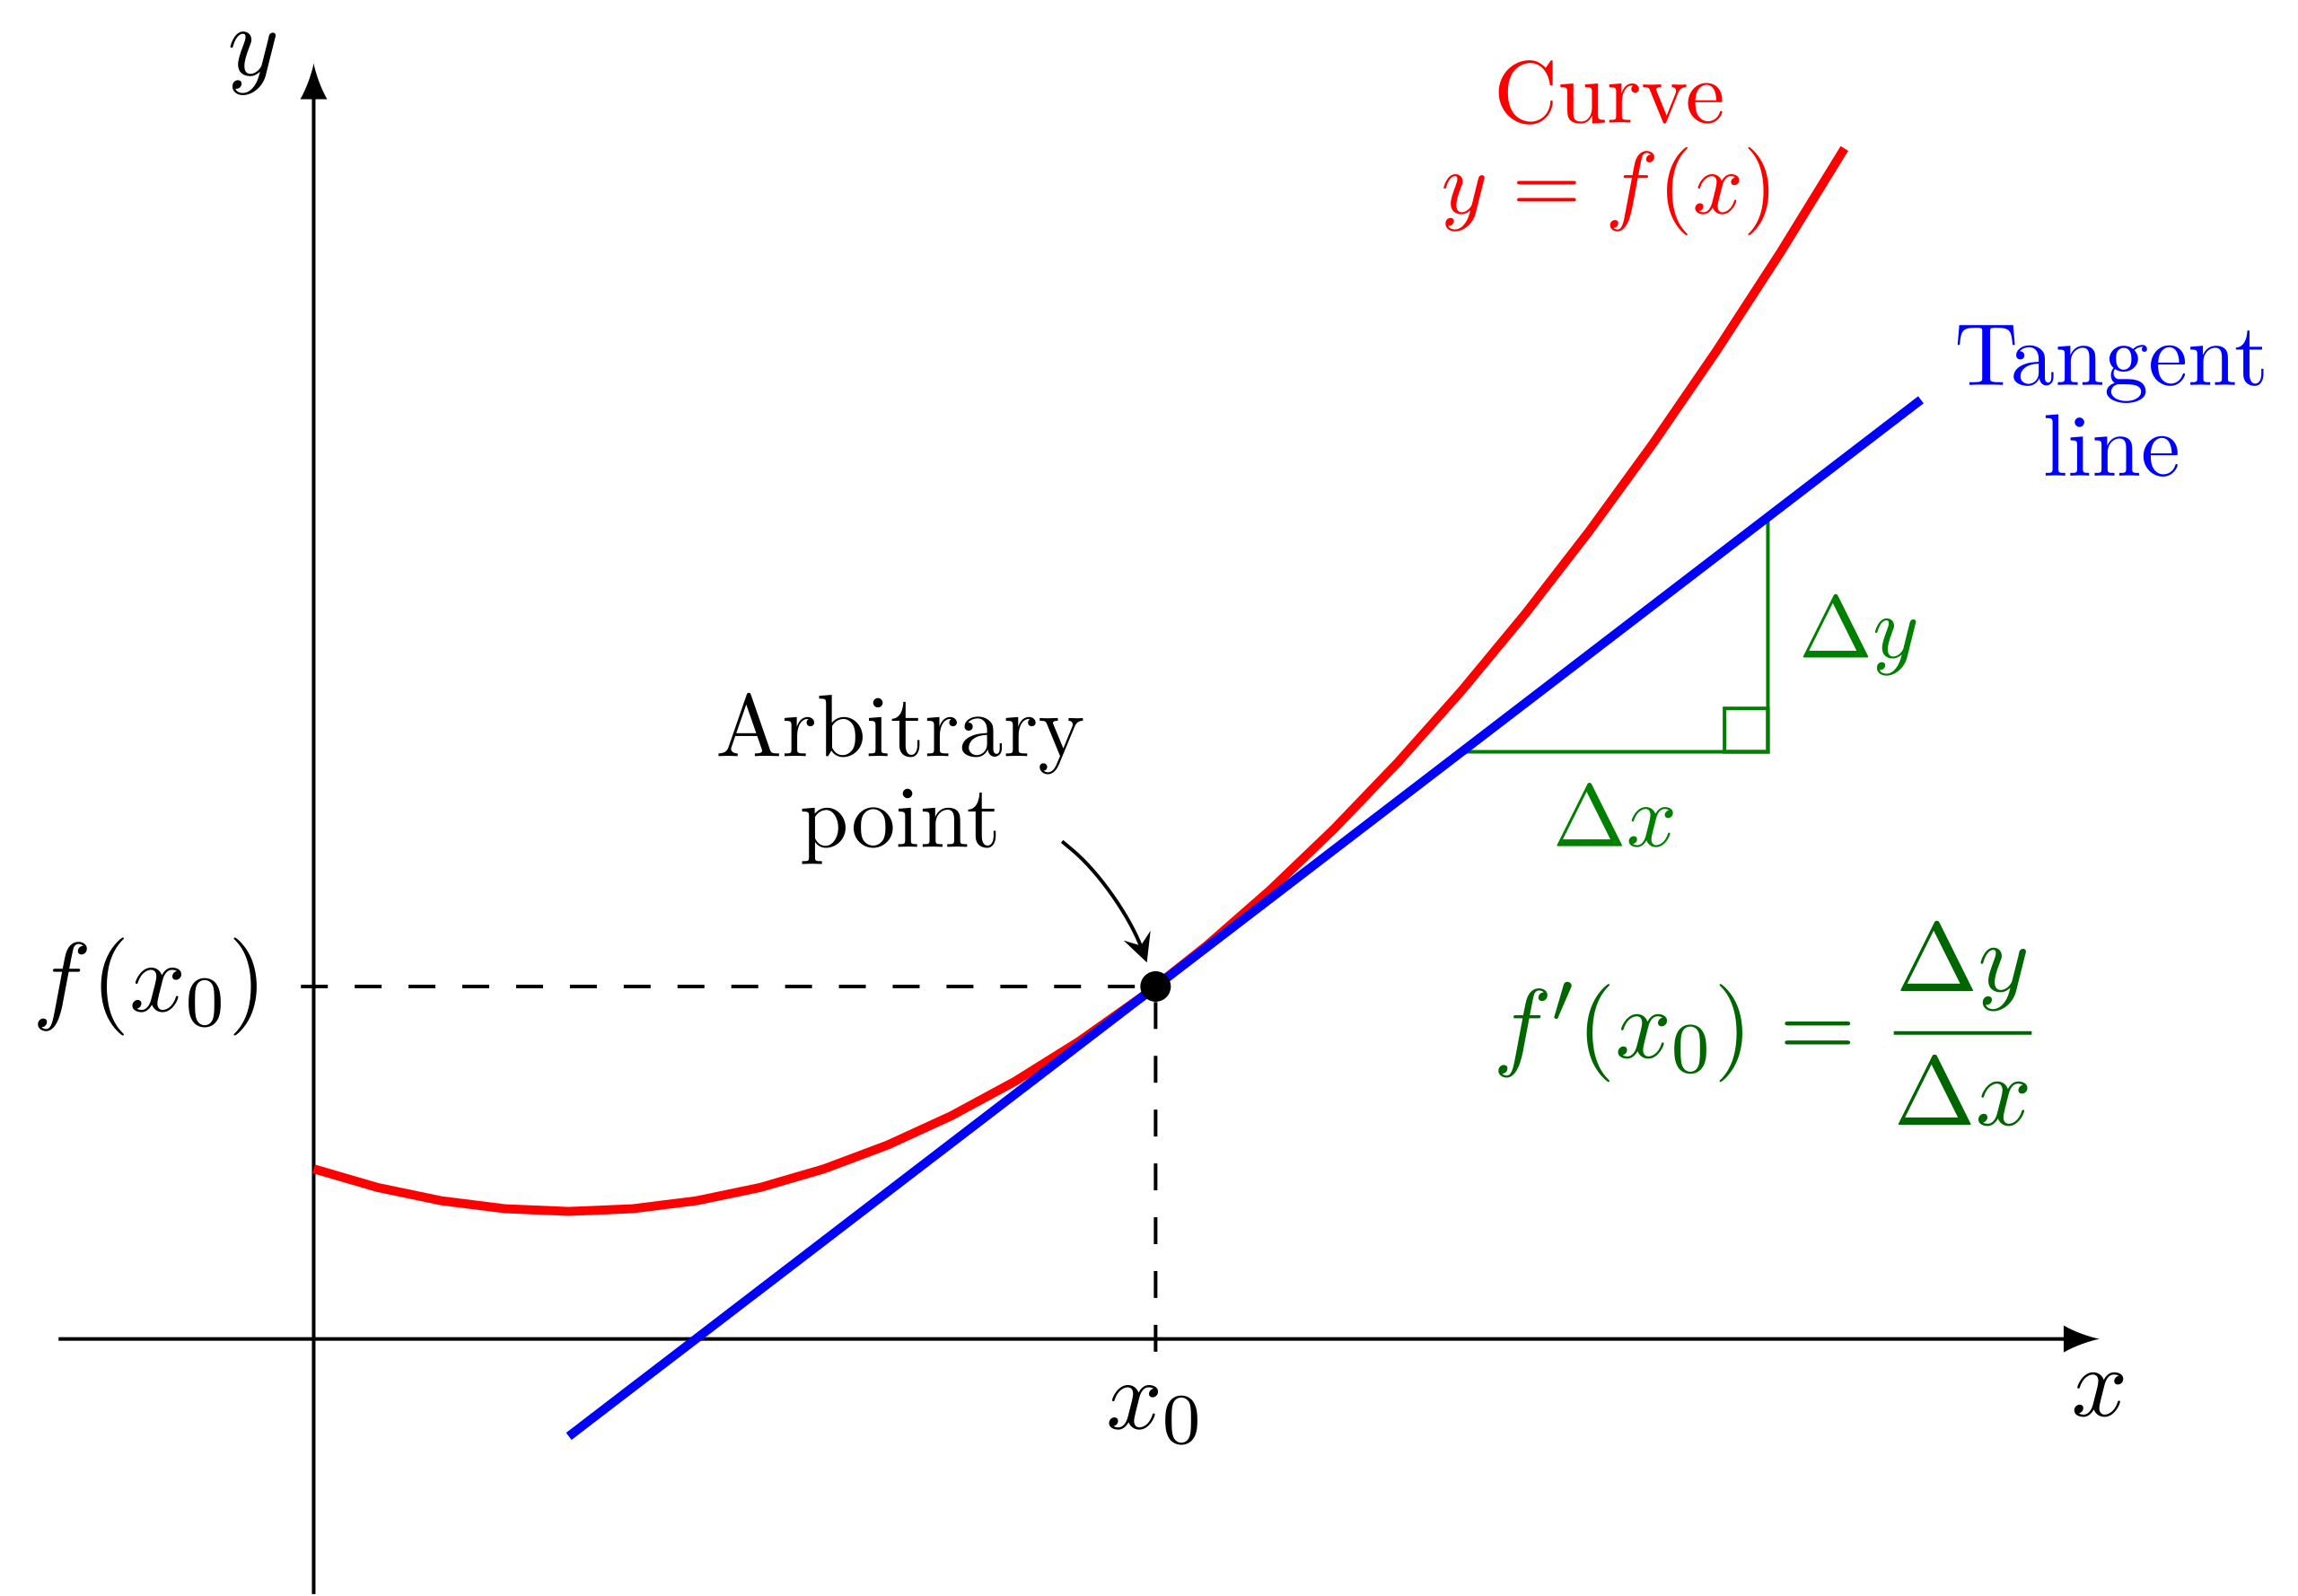
\includegraphics[width=.5\textwidth]{math1.png}

\scriptsize Source: \url{https://commons.wikimedia.org/wiki/File:Tangent_line_to_a_curve.svg}
\caption{Tangent line to a curve}
\label{fig:math1}
\end{figure}

For example, the derivative of the function $f(x) = x^2$ with respect to variable $x$ is written as $f'(x)$ or as $\frac{df}{dx}$ and defined as $f'(x) = \frac{df}{dx} = 2x$. Therefore, the slope at point $x=1$ is $f'(1) = 2$ and the slope at point $x=2$ is $f'(2) = 4$. This evaluation of the derivative at a value $x_0$ for a variable $x$ is sometimes written as $\frac{df}{dx}\rvert_{x=x_0}$. 

Table~\ref{tab:math1} lists a number of commonly used derivatives and Table~\ref{tab:math2} lists some useful rules for computing derivatives for combinations of functions.

\begin{table}
\centering
\renewcommand{\arraystretch}{1.25}

\begin{tabular}{|c|c|} \hline
\textbf{Function f} & \textbf{Derivative f'} \\ \hline
$a$ & $0$ \\ \hline
$a x$ & $a$  \\ \hline
$x^p$ & $p x^{p-1}$ \\ \hline
$\sin(x)$ & $\cos(x)$ \\ \hline
$\cos(x)$ & $-\sin(x)$ \\ \hline
$e^x$ & $e^x$ \\ \hline
$\ln(x)$ & $\frac{1}{x}$ \\ \hline
\end{tabular}
\caption{Derivatives of common functions}
\label{tab:math1}
\end{table}

\begin{table}
\centering
\renewcommand{\arraystretch}{1.75}

\begin{tabularx}{\linewidth}{|c|X|} \hline
$(a f + b g)' = a f' + b g'$ & Sum rule for functions $f$ and $g$ with scalars $a$ and $b$ \\ \hline
$(f g)' = f g' + f' g$ & Product rule for functions $f$ and $g$ \\ \hline
$\left(\frac{f}{g}\right)' = \frac{f'g - fg'}{g^2}$ & Quotient rule for functions $f$ and $g$ where $g \neq 0$ \\ \hline
$(h(g(x)))' = h'(g(x)) g'(x)$ & Chain rule for composite functions \\ \hline
\end{tabularx}
\caption{Rules for derivatives}
\label{tab:math2}
\end{table}

When dealing with functions of multiple variables, e.g. $f(x_1, x_2, \ldots , x_n)$ one can take the derivative with respect to each variable, treating the other variables as constants. Such derivatives are called \emph{partial derivatives}\index{Partial derivative} and are written as $\frac{\partial f}{\partial x}$. 

For example, consider the function $f(x_1, x_2) = x_1^2 + x_1 x_2^2$. Then, the two partial derivatives are:

\begin{align*}
\frac{\partial f}{\partial x_1} &= 2 x_1 + x_2^2 \qquad &\text{(treating $x_2$ as a constant)} \\
\frac{\partial f}{\partial x_2} &= 2 x_1 x_2 \qquad &\text{(treating $x_1$ as a constant)}
\end{align*}

These partial derivatives can be written in vector form. This vector is called the \emph{gradient}\index{Gradient} of the function $f$, written using the ''nabla'' symbol $\nabla$:

\begin{align}
\nabla f = \begin{pmatrix}
2 x_1 + x_2^2 \\
2 x_1 x_2 \end{pmatrix} \label{eq:math:gradient}
\end{align}

Evaluating the gradient at some point, for example at $x_1=1, x_2=2$ provides the slope in the $x_1$ and $x_2$ directions at that point:

\begin{align*}
\nabla f \rvert_{x_1=1, x_2=2} = \begin{pmatrix}
2 \cdot 1 + 2^2 \\
2 \cdot 1 \cdot 2 \end{pmatrix} = \begin{pmatrix} 6 \\ 4 \end{pmatrix}
\end{align*}

Gradients can be applied not only to functions of scalars, but also to functions of vectors and matrices. The following identities are useful when working with derivatives of vectors and matrices:

\begin{align*}
\intertext{for vectors $\mathbf{x}$:}
\frac{\partial (\mathbf{a}^T\mathbf{x})}{\partial \mathbf{x}} &= \mathbf{a} \\ 
\frac{\partial (\mathbf{b}^T\mathbf{A} \mathbf{x})}{\partial \mathbf{x}} &= \mathbf{A}^T \mathbf{b} \\ 
\frac{\partial (\mathbf{x}^T\mathbf{A} \mathbf{x})}{\partial \mathbf{x}} &= (\mathbf{A} + \mathbf{A}^T) \mathbf{x} \\
\intertext{for matrices $\mathbf{X}$:}
\frac{\partial (\mathbf{a}^T\mathbf{X} \mathbf{b})}{\partial \mathbf{X}} &= \mathbf{a} \mathbf{b}^T \\
\frac{\partial (\mathbf{a}^T\mathbf{X^T} \mathbf{b})}{\partial \mathbf{X}} &= \mathbf{b} \mathbf{a}^T
\end{align*}

Finally, the \emph{Hessian}\index{Hessian} $\mathbf{H}$ of a function $f$ is the matrix of second partial derivatives. In other words, form the partial derivatives of each partial derivative in the gradient vector; that is, form the partial derivative for each element of the gradient vector. For example, from the gradient in Equation~\ref{eq:math:gradient} one can compute the following Hessian:

\begin{align*}
\mathbf{H}(f) = \begin{pmatrix}
\frac{\partial^2 f}{\partial x_1^2} & \frac{\partial^2 f}{\partial x_1 \partial x_2} \\
\frac{\partial^2 f}{\partial x_2 \partial x_1} & \frac{\partial^2 f}{\partial x_2^2}
\end{pmatrix} = 
\begin{pmatrix}
2 & 2x_2 \\
2 x_2 & 2 x_1 \end{pmatrix}
\end{align*}

